% Options for packages loaded elsewhere
\PassOptionsToPackage{unicode}{hyperref}
\PassOptionsToPackage{hyphens}{url}
\PassOptionsToPackage{dvipsnames,svgnames,x11names}{xcolor}
%
\documentclass[
  letterpaper,
  DIV=11,
  numbers=noendperiod]{scrartcl}

\usepackage{amsmath,amssymb}
\usepackage{iftex}
\ifPDFTeX
  \usepackage[T1]{fontenc}
  \usepackage[utf8]{inputenc}
  \usepackage{textcomp} % provide euro and other symbols
\else % if luatex or xetex
  \usepackage{unicode-math}
  \defaultfontfeatures{Scale=MatchLowercase}
  \defaultfontfeatures[\rmfamily]{Ligatures=TeX,Scale=1}
\fi
\usepackage{lmodern}
\ifPDFTeX\else  
    % xetex/luatex font selection
\fi
% Use upquote if available, for straight quotes in verbatim environments
\IfFileExists{upquote.sty}{\usepackage{upquote}}{}
\IfFileExists{microtype.sty}{% use microtype if available
  \usepackage[]{microtype}
  \UseMicrotypeSet[protrusion]{basicmath} % disable protrusion for tt fonts
}{}
\makeatletter
\@ifundefined{KOMAClassName}{% if non-KOMA class
  \IfFileExists{parskip.sty}{%
    \usepackage{parskip}
  }{% else
    \setlength{\parindent}{0pt}
    \setlength{\parskip}{6pt plus 2pt minus 1pt}}
}{% if KOMA class
  \KOMAoptions{parskip=half}}
\makeatother
\usepackage{xcolor}
\usepackage{svg}
\ifLuaTeX
  \usepackage{luacolor}
  \usepackage[soul]{lua-ul}
\else
  \usepackage{soul}
  
\fi
\setlength{\emergencystretch}{3em} % prevent overfull lines
\setcounter{secnumdepth}{-\maxdimen} % remove section numbering
% Make \paragraph and \subparagraph free-standing
\makeatletter
\ifx\paragraph\undefined\else
  \let\oldparagraph\paragraph
  \renewcommand{\paragraph}{
    \@ifstar
      \xxxParagraphStar
      \xxxParagraphNoStar
  }
  \newcommand{\xxxParagraphStar}[1]{\oldparagraph*{#1}\mbox{}}
  \newcommand{\xxxParagraphNoStar}[1]{\oldparagraph{#1}\mbox{}}
\fi
\ifx\subparagraph\undefined\else
  \let\oldsubparagraph\subparagraph
  \renewcommand{\subparagraph}{
    \@ifstar
      \xxxSubParagraphStar
      \xxxSubParagraphNoStar
  }
  \newcommand{\xxxSubParagraphStar}[1]{\oldsubparagraph*{#1}\mbox{}}
  \newcommand{\xxxSubParagraphNoStar}[1]{\oldsubparagraph{#1}\mbox{}}
\fi
\makeatother

\usepackage{color}
\usepackage{fancyvrb}
\newcommand{\VerbBar}{|}
\newcommand{\VERB}{\Verb[commandchars=\\\{\}]}
\DefineVerbatimEnvironment{Highlighting}{Verbatim}{commandchars=\\\{\}}
% Add ',fontsize=\small' for more characters per line
\usepackage{framed}
\definecolor{shadecolor}{RGB}{241,243,245}
\newenvironment{Shaded}{\begin{snugshade}}{\end{snugshade}}
\newcommand{\AlertTok}[1]{\textcolor[rgb]{0.68,0.00,0.00}{#1}}
\newcommand{\AnnotationTok}[1]{\textcolor[rgb]{0.37,0.37,0.37}{#1}}
\newcommand{\AttributeTok}[1]{\textcolor[rgb]{0.40,0.45,0.13}{#1}}
\newcommand{\BaseNTok}[1]{\textcolor[rgb]{0.68,0.00,0.00}{#1}}
\newcommand{\BuiltInTok}[1]{\textcolor[rgb]{0.00,0.23,0.31}{#1}}
\newcommand{\CharTok}[1]{\textcolor[rgb]{0.13,0.47,0.30}{#1}}
\newcommand{\CommentTok}[1]{\textcolor[rgb]{0.37,0.37,0.37}{#1}}
\newcommand{\CommentVarTok}[1]{\textcolor[rgb]{0.37,0.37,0.37}{\textit{#1}}}
\newcommand{\ConstantTok}[1]{\textcolor[rgb]{0.56,0.35,0.01}{#1}}
\newcommand{\ControlFlowTok}[1]{\textcolor[rgb]{0.00,0.23,0.31}{\textbf{#1}}}
\newcommand{\DataTypeTok}[1]{\textcolor[rgb]{0.68,0.00,0.00}{#1}}
\newcommand{\DecValTok}[1]{\textcolor[rgb]{0.68,0.00,0.00}{#1}}
\newcommand{\DocumentationTok}[1]{\textcolor[rgb]{0.37,0.37,0.37}{\textit{#1}}}
\newcommand{\ErrorTok}[1]{\textcolor[rgb]{0.68,0.00,0.00}{#1}}
\newcommand{\ExtensionTok}[1]{\textcolor[rgb]{0.00,0.23,0.31}{#1}}
\newcommand{\FloatTok}[1]{\textcolor[rgb]{0.68,0.00,0.00}{#1}}
\newcommand{\FunctionTok}[1]{\textcolor[rgb]{0.28,0.35,0.67}{#1}}
\newcommand{\ImportTok}[1]{\textcolor[rgb]{0.00,0.46,0.62}{#1}}
\newcommand{\InformationTok}[1]{\textcolor[rgb]{0.37,0.37,0.37}{#1}}
\newcommand{\KeywordTok}[1]{\textcolor[rgb]{0.00,0.23,0.31}{\textbf{#1}}}
\newcommand{\NormalTok}[1]{\textcolor[rgb]{0.00,0.23,0.31}{#1}}
\newcommand{\OperatorTok}[1]{\textcolor[rgb]{0.37,0.37,0.37}{#1}}
\newcommand{\OtherTok}[1]{\textcolor[rgb]{0.00,0.23,0.31}{#1}}
\newcommand{\PreprocessorTok}[1]{\textcolor[rgb]{0.68,0.00,0.00}{#1}}
\newcommand{\RegionMarkerTok}[1]{\textcolor[rgb]{0.00,0.23,0.31}{#1}}
\newcommand{\SpecialCharTok}[1]{\textcolor[rgb]{0.37,0.37,0.37}{#1}}
\newcommand{\SpecialStringTok}[1]{\textcolor[rgb]{0.13,0.47,0.30}{#1}}
\newcommand{\StringTok}[1]{\textcolor[rgb]{0.13,0.47,0.30}{#1}}
\newcommand{\VariableTok}[1]{\textcolor[rgb]{0.07,0.07,0.07}{#1}}
\newcommand{\VerbatimStringTok}[1]{\textcolor[rgb]{0.13,0.47,0.30}{#1}}
\newcommand{\WarningTok}[1]{\textcolor[rgb]{0.37,0.37,0.37}{\textit{#1}}}

\providecommand{\tightlist}{%
  \setlength{\itemsep}{0pt}\setlength{\parskip}{0pt}}\usepackage{longtable,booktabs,array}
\usepackage{calc} % for calculating minipage widths
% Correct order of tables after \paragraph or \subparagraph
\usepackage{etoolbox}
\makeatletter
\patchcmd\longtable{\par}{\if@noskipsec\mbox{}\fi\par}{}{}
\makeatother
% Allow footnotes in longtable head/foot
\IfFileExists{footnotehyper.sty}{\usepackage{footnotehyper}}{\usepackage{footnote}}
\makesavenoteenv{longtable}
\usepackage{graphicx}
\makeatletter
\def\maxwidth{\ifdim\Gin@nat@width>\linewidth\linewidth\else\Gin@nat@width\fi}
\def\maxheight{\ifdim\Gin@nat@height>\textheight\textheight\else\Gin@nat@height\fi}
\makeatother
% Scale images if necessary, so that they will not overflow the page
% margins by default, and it is still possible to overwrite the defaults
% using explicit options in \includegraphics[width, height, ...]{}
\setkeys{Gin}{width=\maxwidth,height=\maxheight,keepaspectratio}
% Set default figure placement to htbp
\makeatletter
\def\fps@figure{htbp}
\makeatother

\KOMAoption{captions}{tableheading}
\makeatletter
\@ifpackageloaded{caption}{}{\usepackage{caption}}
\AtBeginDocument{%
\ifdefined\contentsname
  \renewcommand*\contentsname{Table of contents}
\else
  \newcommand\contentsname{Table of contents}
\fi
\ifdefined\listfigurename
  \renewcommand*\listfigurename{List of Figures}
\else
  \newcommand\listfigurename{List of Figures}
\fi
\ifdefined\listtablename
  \renewcommand*\listtablename{List of Tables}
\else
  \newcommand\listtablename{List of Tables}
\fi
\ifdefined\figurename
  \renewcommand*\figurename{Figure}
\else
  \newcommand\figurename{Figure}
\fi
\ifdefined\tablename
  \renewcommand*\tablename{Table}
\else
  \newcommand\tablename{Table}
\fi
}
\@ifpackageloaded{float}{}{\usepackage{float}}
\floatstyle{ruled}
\@ifundefined{c@chapter}{\newfloat{codelisting}{h}{lop}}{\newfloat{codelisting}{h}{lop}[chapter]}
\floatname{codelisting}{Listing}
\newcommand*\listoflistings{\listof{codelisting}{List of Listings}}
\makeatother
\makeatletter
\makeatother
\makeatletter
\@ifpackageloaded{caption}{}{\usepackage{caption}}
\@ifpackageloaded{subcaption}{}{\usepackage{subcaption}}
\makeatother

\ifLuaTeX
  \usepackage{selnolig}  % disable illegal ligatures
\fi
\usepackage{bookmark}

\IfFileExists{xurl.sty}{\usepackage{xurl}}{} % add URL line breaks if available
\urlstyle{same} % disable monospaced font for URLs
\hypersetup{
  colorlinks=true,
  linkcolor={blue},
  filecolor={Maroon},
  citecolor={Blue},
  urlcolor={Blue},
  pdfcreator={LaTeX via pandoc}}


\author{}
\date{}

\begin{document}


\includesvg[width=2.60417in,height=\textheight]{Demo_guide_files/mediabag/logo.svg}

\section{\texorpdfstring{\ul{Geomatching}: a sneak
peek}{Geomatching: a sneak peek}}\label{geomatching-a-sneak-peek}

\subsection{Import R libraries}\label{import-r-libraries}

\begin{Shaded}
\begin{Highlighting}[]
\FunctionTok{rm}\NormalTok{(}\AttributeTok{list =} \FunctionTok{ls}\NormalTok{())}
\FunctionTok{library}\NormalTok{(ggplot2)}
\FunctionTok{library}\NormalTok{(mapdata)}
\end{Highlighting}
\end{Shaded}

\begin{verbatim}
Loading required package: maps
\end{verbatim}

\begin{Shaded}
\begin{Highlighting}[]
\FunctionTok{library}\NormalTok{(geotools)}
\end{Highlighting}
\end{Shaded}

\begin{verbatim}
Loading required package: dplyr
\end{verbatim}

\begin{verbatim}

Attaching package: 'dplyr'
\end{verbatim}

\begin{verbatim}
The following objects are masked from 'package:stats':

    filter, lag
\end{verbatim}

\begin{verbatim}
The following objects are masked from 'package:base':

    intersect, setdiff, setequal, union
\end{verbatim}

\begin{verbatim}
Loading required package: foreach
\end{verbatim}

\subsection{Import (local) data}\label{import-local-data}

\begin{itemize}
\item
  \texttt{ERA5Land\_t2m\_10d}: time-spatial data.frame
  (\emph{longitude}, \emph{latitude} and \emph{time}) containing 10 days
  of \textbf{air temperature}. Grid resolution: 0.1° x 0.1° (about 11 km
  x 11 km).
\item
  \texttt{ERA5SL\_t2m\_10d}: time-spatial data.frame containing 10 days
  of \textbf{air temperature}. Grid resolution: 0.25° x 0.25° (about 27
  km x 27 km).
\item
  \texttt{ERA5SL\_rh\_10d}: time-spatial data.frame containing 10 days
  of \textbf{relative humidity}. Grid resolution: 0.25° x 0.25° (about
  27 km x 27 km).
\item
  \texttt{ERA5SL\_lai\_hv\_10d\_matrix}: 3D matrix (\emph{x}-component
  represents \emph{longitude, y}-component describes \emph{latitude} and
  \emph{z-}component represents \emph{time}) 10 days of \textbf{Leaf
  Area Index - High Vegetation}. Grid resolution: 0.25° x 0.25° (about
  27 km x 27 km).
\end{itemize}

\begin{Shaded}
\begin{Highlighting}[]
\CommentTok{\# weather data}
\FunctionTok{load}\NormalTok{(}\StringTok{"WE\_raw\_data.Rdata"}\NormalTok{)}
\FunctionTok{names}\NormalTok{(ERA5Land\_t2m\_10d)[}\DecValTok{4}\NormalTok{] }\OtherTok{\textless{}{-}} \StringTok{"t2m\_Land"}
\FunctionTok{names}\NormalTok{(ERA5SL\_t2m\_10d)[}\DecValTok{4}\NormalTok{] }\OtherTok{\textless{}{-}} \StringTok{"t2m\_SL"}
\NormalTok{WE\_data }\OtherTok{=} \FunctionTok{list}\NormalTok{(}
  \StringTok{"ERA5Land\_t2m"} \OtherTok{=} \FunctionTok{list}\NormalTok{(}
    \StringTok{"data"} \OtherTok{=}\NormalTok{ ERA5Land\_t2m\_10d,}
    \StringTok{"var"} \OtherTok{=} \StringTok{"t2m\_Land"}\NormalTok{,}
    \StringTok{"label"} \OtherTok{=} \StringTok{"Air temperature, ERA5Land (11 km x 11 km)"}
\NormalTok{  ),}
  \StringTok{"ERA5SL\_t2m"} \OtherTok{=} \FunctionTok{list}\NormalTok{(}
    \StringTok{"data"} \OtherTok{=}\NormalTok{ ERA5SL\_t2m\_10d,}
    \StringTok{"var"} \OtherTok{=} \StringTok{"t2m\_SL"}\NormalTok{,}
    \StringTok{"label"} \OtherTok{=} \StringTok{"Air temperature, ERA5SL (27 km x 27 km)"}
\NormalTok{  ),}
  \StringTok{"ERA5SL\_rh"} \OtherTok{=} \FunctionTok{list}\NormalTok{(}
    \StringTok{"data"} \OtherTok{=}\NormalTok{ ERA5SL\_rh\_10d,}
    \StringTok{"var"} \OtherTok{=} \StringTok{"rh"}\NormalTok{,}
    \StringTok{"label"} \OtherTok{=} \StringTok{"Relative humidity, ERA5SL (27 km x 27 km)"}
\NormalTok{  )}
\NormalTok{)}

\CommentTok{\# LAUs boundaries}
\FunctionTok{names}\NormalTok{(mun\_bounds)[}\DecValTok{6}\NormalTok{] }\OtherTok{\textless{}{-}} \StringTok{"COD\_COM"}
\NormalTok{LAUs\_data }\OtherTok{=} \FunctionTok{list}\NormalTok{(}
  \StringTok{"mun\_bounds"} \OtherTok{=} \FunctionTok{list}\NormalTok{(}
    \StringTok{"data"} \OtherTok{=}\NormalTok{ geotools}\SpecialCharTok{::}\NormalTok{mun\_bounds,}
    \StringTok{"code"} \OtherTok{=} \StringTok{"mun"}\NormalTok{,}
    \StringTok{"join\_var"} \OtherTok{=} \StringTok{"PRO\_COM"}
\NormalTok{  ),}
  \StringTok{"prov\_bounds"} \OtherTok{=} \FunctionTok{list}\NormalTok{(}
    \StringTok{"data"} \OtherTok{=}\NormalTok{ geotools}\SpecialCharTok{::}\NormalTok{prov\_bounds,}
    \StringTok{"code"} \OtherTok{=} \StringTok{"prov"}\NormalTok{,}
    \StringTok{"join\_var"} \OtherTok{=} \StringTok{"COD\_PROV"}
\NormalTok{  ),}
  \StringTok{"reg\_bounds"} \OtherTok{=} \FunctionTok{list}\NormalTok{(}
    \StringTok{"data"} \OtherTok{=}\NormalTok{ geotools}\SpecialCharTok{::}\NormalTok{reg\_bounds,}
    \StringTok{"code"} \OtherTok{=} \StringTok{"reg"}\NormalTok{,}
    \StringTok{"join\_var"} \OtherTok{=} \StringTok{"COD\_REG"}
\NormalTok{  )}
\NormalTok{)}
\end{Highlighting}
\end{Shaded}

\subsubsection{Visualize first rows of each
data.frame}\label{visualize-first-rows-of-each-data.frame}

\texttt{ERA5Land\_t2m\_10d}

\begin{Shaded}
\begin{Highlighting}[]
\FunctionTok{head}\NormalTok{(ERA5Land\_t2m\_10d, }\AttributeTok{n =} \DecValTok{10}\NormalTok{)}
\end{Highlighting}
\end{Shaded}

\begin{verbatim}
   longitude latitude       time t2m_Land
1          6     48.0 2013-01-01 5.308351
2          6     47.9 2013-01-01 5.617759
3          6     47.8 2013-01-01 5.829429
4          6     47.7 2013-01-01 6.035239
5          6     47.6 2013-01-01 6.123781
6          6     47.5 2013-01-01 6.104250
7          6     47.4 2013-01-01 6.273520
8          6     47.3 2013-01-01 6.243166
9          6     47.2 2013-01-01 5.943280
10         6     47.1 2013-01-01 5.592205
\end{verbatim}

\texttt{ERA5SL\_t2m\_10d}

\begin{Shaded}
\begin{Highlighting}[]
\FunctionTok{head}\NormalTok{(ERA5SL\_t2m\_10d, }\AttributeTok{n =} \DecValTok{10}\NormalTok{)}
\end{Highlighting}
\end{Shaded}

\begin{verbatim}
   longitude latitude       time   t2m_SL
1          6    48.00 2013-01-01 5.631985
2          6    47.75 2013-01-01 6.295315
3          6    47.50 2013-01-01 6.754544
4          6    47.25 2013-01-01 6.592516
5          6    47.00 2013-01-01 5.405178
6          6    46.75 2013-01-01 3.390530
7          6    46.50 2013-01-01 2.423489
8          6    46.25 2013-01-01 2.588853
9          6    46.00 2013-01-01 2.084459
10         6    45.75 2013-01-01 1.991034
\end{verbatim}

\texttt{ERA5SL\_rh\_10d}

\begin{Shaded}
\begin{Highlighting}[]
\FunctionTok{head}\NormalTok{(ERA5SL\_rh\_10d, }\AttributeTok{n =} \DecValTok{10}\NormalTok{)}
\end{Highlighting}
\end{Shaded}

\begin{verbatim}
   longitude latitude       time       rh
1       6.00       48 2013-01-01 88.84715
2       6.25       48 2013-01-01 87.67344
3       6.50       48 2013-01-01 86.28634
4       6.75       48 2013-01-01 85.53499
5       7.00       48 2013-01-01 86.53418
6       7.25       48 2013-01-01 90.22042
7       7.50       48 2013-01-01 92.99447
8       7.75       48 2013-01-01 93.77895
9       8.00       48 2013-01-01 89.41314
10      8.25       48 2013-01-01 83.32842
\end{verbatim}

\subsection{First look}\label{first-look}

\begin{Shaded}
\begin{Highlighting}[]
\ControlFlowTok{for}\NormalTok{ (item\_i }\ControlFlowTok{in}\NormalTok{ WE\_data) \{}
  
  \CommentTok{\# configuration}
\NormalTok{  df\_i }\OtherTok{\textless{}{-}}\NormalTok{ item\_i}\SpecialCharTok{$}\NormalTok{data}
\NormalTok{  var\_i }\OtherTok{\textless{}{-}}\NormalTok{ item\_i}\SpecialCharTok{$}\NormalTok{var}
\NormalTok{  label\_i }\OtherTok{\textless{}{-}}\NormalTok{ item\_i}\SpecialCharTok{$}\NormalTok{label}
\NormalTok{  subset\_i }\OtherTok{\textless{}{-}}\NormalTok{ df\_i[df\_i}\SpecialCharTok{$}\NormalTok{time }\SpecialCharTok{==}\NormalTok{ df\_i}\SpecialCharTok{$}\NormalTok{time[}\DecValTok{1}\NormalTok{], ]}
  
  \CommentTok{\# run}
\NormalTok{  p }\OtherTok{\textless{}{-}} \FunctionTok{ggplot}\NormalTok{() }\SpecialCharTok{+}
    \FunctionTok{geom\_map}\NormalTok{(}
      \AttributeTok{data =} \FunctionTok{map\_data}\NormalTok{(}\StringTok{"italy"}\NormalTok{),}
      \AttributeTok{map =} \FunctionTok{map\_data}\NormalTok{(}\StringTok{"italy"}\NormalTok{),}
      \FunctionTok{aes}\NormalTok{(}\AttributeTok{map\_id =}\NormalTok{ region),}
      \AttributeTok{fill =} \StringTok{"lightgrey"}\NormalTok{,}
      \AttributeTok{color =} \StringTok{"black"}\NormalTok{,}
      \AttributeTok{linewidth =}\NormalTok{ .}\DecValTok{1}\NormalTok{,}
      \AttributeTok{alpha=}\NormalTok{.}\DecValTok{9}
\NormalTok{    ) }\SpecialCharTok{+} 
    \FunctionTok{geom\_tile}\NormalTok{(}
      \AttributeTok{data =}\NormalTok{ subset\_i,}
      \FunctionTok{aes}\NormalTok{(}\AttributeTok{x =}\NormalTok{ longitude, }\AttributeTok{y =}\NormalTok{ latitude, }\AttributeTok{fill =}\NormalTok{ .data[[var\_i]])}
\NormalTok{    ) }\SpecialCharTok{+}
    \FunctionTok{labs}\NormalTok{(}
      \AttributeTok{title =} \FunctionTok{sprintf}\NormalTok{(}\StringTok{"Geographical map of weather data"}\NormalTok{),}
      \AttributeTok{subtitle =}\NormalTok{ label\_i,}
      \AttributeTok{x =} \StringTok{"Longitude"}\NormalTok{,}
      \AttributeTok{y =} \StringTok{"Latitude"}
\NormalTok{    ) }\SpecialCharTok{+} 
    \FunctionTok{scale\_fill\_viridis\_c}\NormalTok{(}
      \AttributeTok{option =} \StringTok{"C"}
\NormalTok{    ) }\SpecialCharTok{+}
    \FunctionTok{theme}\NormalTok{(}
      \AttributeTok{legend.title =} \FunctionTok{element\_blank}\NormalTok{(),}
      \AttributeTok{plot.title =} \FunctionTok{element\_text}\NormalTok{(}\AttributeTok{face =} \StringTok{"bold"}\NormalTok{)}
\NormalTok{    )}
  \FunctionTok{print}\NormalTok{(p)}
\NormalTok{\}}
\end{Highlighting}
\end{Shaded}

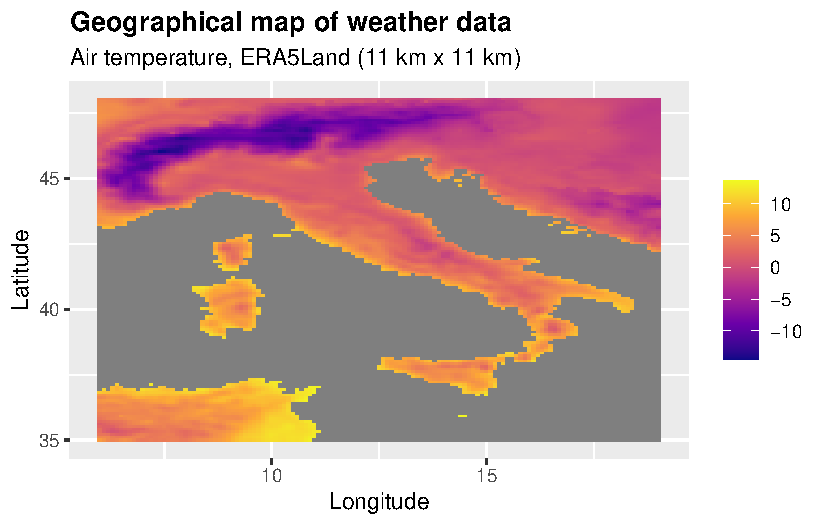
\includegraphics{Demo_guide_files/figure-pdf/unnamed-chunk-6-1.pdf}

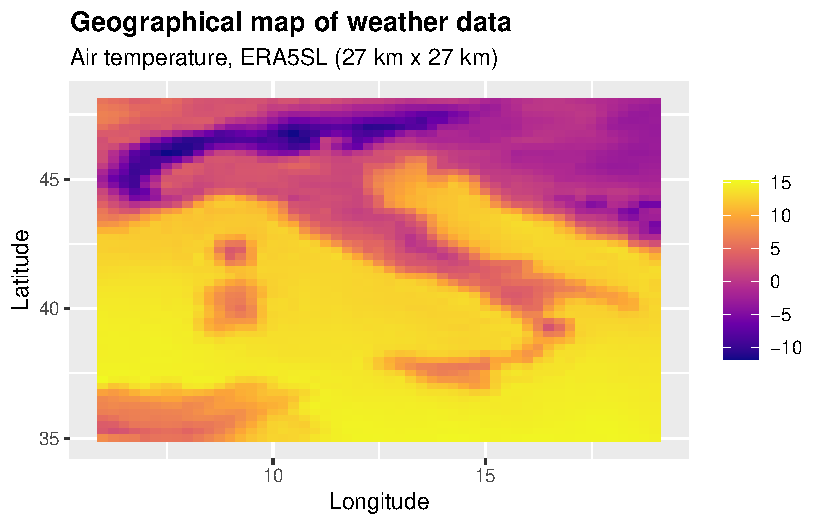
\includegraphics{Demo_guide_files/figure-pdf/unnamed-chunk-6-2.pdf}

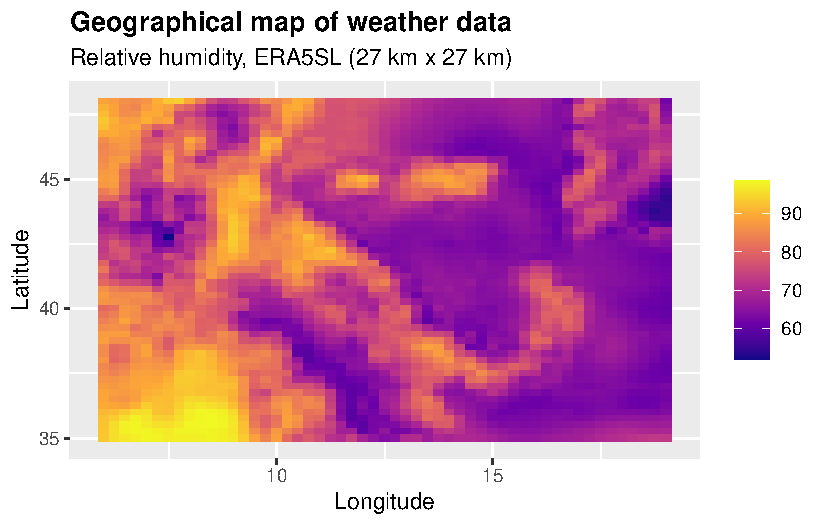
\includegraphics{Demo_guide_files/figure-pdf/unnamed-chunk-6-3.pdf}

\subsection{Run geomatching}\label{run-geomatching}

\begin{Shaded}
\begin{Highlighting}[]
\NormalTok{aggr\_data }\OtherTok{\textless{}{-}} \FunctionTok{list}\NormalTok{()}
\ControlFlowTok{for}\NormalTok{ (item\_i }\ControlFlowTok{in}\NormalTok{ LAUs\_data) \{}
  
  \CommentTok{\# configuration}
\NormalTok{  bounds\_i }\OtherTok{\textless{}{-}}\NormalTok{ item\_i}\SpecialCharTok{$}\NormalTok{data}
\NormalTok{  code\_i }\OtherTok{\textless{}{-}}\NormalTok{ item\_i}\SpecialCharTok{$}\NormalTok{code}
\NormalTok{  join\_var\_i }\OtherTok{\textless{}{-}}\NormalTok{ item\_i}\SpecialCharTok{$}\NormalTok{join\_var}
  
  \CommentTok{\# run}
\NormalTok{  temp }\OtherTok{\textless{}{-}}\NormalTok{ geotools}\SpecialCharTok{::}\FunctionTok{geomatching}\NormalTok{(}
    \AttributeTok{data =} \FunctionTok{list}\NormalTok{(}
\NormalTok{      ERA5Land\_t2m\_10d,}
\NormalTok{      ERA5SL\_t2m\_10d,}
\NormalTok{      ERA5SL\_rh\_10d,}
\NormalTok{      ERA5SL\_lai\_hv\_10d\_matrix}
\NormalTok{    ),}
    \AttributeTok{settings =} \FunctionTok{list}\NormalTok{(}
      \StringTok{"format"} \OtherTok{=} \FunctionTok{list}\NormalTok{(}
        \StringTok{"xyt"}\NormalTok{,}
        \StringTok{"xyt"}\NormalTok{,}
        \StringTok{"xyt"}\NormalTok{,}
        \StringTok{"matrix"}
\NormalTok{      ),}
      \StringTok{"type"} \OtherTok{=} \FunctionTok{list}\NormalTok{(}
        \StringTok{"grid"}\NormalTok{,}
        \StringTok{"grid"}\NormalTok{,}
        \StringTok{"grid"}\NormalTok{,}
        \StringTok{"grid"}
\NormalTok{      ),}
      \StringTok{"crs"} \OtherTok{=} \FunctionTok{list}\NormalTok{(}
        \DecValTok{4326}\NormalTok{,}
        \DecValTok{4326}\NormalTok{,}
        \DecValTok{4326}\NormalTok{,}
        \DecValTok{4326}
\NormalTok{      )}
\NormalTok{    ),}
    \AttributeTok{aggregate =} \ConstantTok{TRUE}\NormalTok{,}
    \AttributeTok{group\_by =}\NormalTok{ code\_i}
\NormalTok{  )}
  
  \CommentTok{\# rename columns \#1}
  \FunctionTok{names}\NormalTok{(temp)[}\DecValTok{24}\SpecialCharTok{:}\DecValTok{30}\NormalTok{] }\OtherTok{\textless{}{-}} \FunctionTok{c}\NormalTok{(}
    \StringTok{"lai\_hv\_min"}\NormalTok{,}
    \StringTok{"lai\_hv\_1st\_quartile"}\NormalTok{,}
    \StringTok{"lai\_hv\_mean"}\NormalTok{,}
    \StringTok{"lai\_hv\_median"}\NormalTok{,}
    \StringTok{"lai\_hv\_3rd\_quartile"}\NormalTok{,}
    \StringTok{"lai\_hv\_max"}\NormalTok{,}
    \StringTok{"lai\_hv\_std"}
\NormalTok{  )}
  
  \CommentTok{\# fill missing values}
\NormalTok{  stats }\OtherTok{\textless{}{-}} \FunctionTok{c}\NormalTok{(}\StringTok{"min"}\NormalTok{, }\StringTok{"1st\_quartile"}\NormalTok{, }\StringTok{"mean"}\NormalTok{, }\StringTok{"median"}\NormalTok{, }\StringTok{"3rd\_quartile"}\NormalTok{, }\StringTok{"max"}\NormalTok{, }\StringTok{"std"}\NormalTok{)}
  \ControlFlowTok{for}\NormalTok{ (stat\_i }\ControlFlowTok{in}\NormalTok{ stats) \{}
\NormalTok{    land\_col }\OtherTok{\textless{}{-}} \FunctionTok{paste0}\NormalTok{(}\StringTok{"t2m\_Land\_"}\NormalTok{, stat\_i)}
\NormalTok{    sl\_col }\OtherTok{\textless{}{-}} \FunctionTok{paste0}\NormalTok{(}\StringTok{"t2m\_SL\_"}\NormalTok{, stat\_i)}
\NormalTok{    temp[[land\_col]][}\FunctionTok{is.na}\NormalTok{(temp[[land\_col]])] }\OtherTok{\textless{}{-}}\NormalTok{ temp[[sl\_col]][}\FunctionTok{is.na}\NormalTok{(temp[[land\_col]])]}
\NormalTok{  \}}
  
  \CommentTok{\# drop columns}
\NormalTok{  temp }\OtherTok{\textless{}{-}}\NormalTok{ temp[, }\SpecialCharTok{!}\FunctionTok{names}\NormalTok{(temp) }\SpecialCharTok{\%in\%} \FunctionTok{c}\NormalTok{(}
    \StringTok{"t2m\_SL\_min"}\NormalTok{, }\StringTok{"t2m\_SL\_1st\_quartile"}\NormalTok{, }\StringTok{"t2m\_SL\_mean"}\NormalTok{, }\StringTok{"t2m\_SL\_median"}\NormalTok{,}
    \StringTok{"t2m\_SL\_3rd\_quartile"}\NormalTok{, }\StringTok{"t2m\_SL\_max"}\NormalTok{, }\StringTok{"t2m\_SL\_std"}\NormalTok{)}
\NormalTok{  ]}
  
  \CommentTok{\# rename columns \#2}
  \FunctionTok{names}\NormalTok{(temp)[}\DecValTok{3}\SpecialCharTok{:}\DecValTok{9}\NormalTok{] }\OtherTok{\textless{}{-}} \FunctionTok{c}\NormalTok{(}
    \StringTok{"t2m\_min"}\NormalTok{,}
    \StringTok{"t2m\_1st\_quartile"}\NormalTok{,}
    \StringTok{"t2m\_mean"}\NormalTok{,}
    \StringTok{"t2m\_median"}\NormalTok{,}
    \StringTok{"t2m\_3rd\_quartile"}\NormalTok{,}
    \StringTok{"t2m\_max"}\NormalTok{,}
    \StringTok{"t2m\_std"}
\NormalTok{  )}
  
  \CommentTok{\# join}
\NormalTok{  temp }\OtherTok{\textless{}{-}} \FunctionTok{left\_join}\NormalTok{(}
\NormalTok{    bounds\_i,}
\NormalTok{    temp,}
    \AttributeTok{by =}\NormalTok{ join\_var\_i}
\NormalTok{  )}
  
  \CommentTok{\# save}
\NormalTok{  aggr\_data[[code\_i]] }\OtherTok{\textless{}{-}}\NormalTok{ temp}
\NormalTok{\}}
\end{Highlighting}
\end{Shaded}

\begin{verbatim}
[1] "reading data 1"
[1] "done"
[1] "reading data 2"
[1] "done"
[1] "reading data 3"
[1] "done"
[1] "reading data 4"
[1] "done"
[1] "reading data 5"
[1] "done"
[1] "converting data 1 to ST"
[1] "done"
[1] "converting data 2 to ST"
[1] "done"
[1] "converting data 3 to ST"
[1] "done"
[1] "converting data 4 to ST"
[1] "done"
[1] "converting data 5 to ST"
[1] "done"
[1] "reading data 1"
[1] "done"
[1] "reading data 2"
[1] "done"
[1] "reading data 3"
[1] "done"
[1] "reading data 4"
[1] "done"
[1] "reading data 5"
[1] "done"
[1] "converting data 1 to ST"
[1] "done"
[1] "converting data 2 to ST"
[1] "done"
[1] "converting data 3 to ST"
[1] "done"
[1] "converting data 4 to ST"
[1] "done"
[1] "converting data 5 to ST"
[1] "done"
[1] "reading data 1"
[1] "done"
[1] "reading data 2"
[1] "done"
[1] "reading data 3"
[1] "done"
[1] "reading data 4"
[1] "done"
[1] "reading data 5"
[1] "done"
[1] "converting data 1 to ST"
[1] "done"
[1] "converting data 2 to ST"
[1] "done"
[1] "converting data 3 to ST"
[1] "done"
[1] "converting data 4 to ST"
[1] "done"
[1] "converting data 5 to ST"
[1] "done"
\end{verbatim}

\subsection{Visualize aggregated data}\label{visualize-aggregated-data}

\begin{Shaded}
\begin{Highlighting}[]
\ControlFlowTok{for}\NormalTok{ (code\_i }\ControlFlowTok{in} \FunctionTok{names}\NormalTok{(aggr\_data)) \{}
  
  \CommentTok{\# configuration}
\NormalTok{  df\_i }\OtherTok{\textless{}{-}}\NormalTok{ aggr\_data[[code\_i]]}
\NormalTok{  subset\_i }\OtherTok{\textless{}{-}}\NormalTok{ df\_i[df\_i}\SpecialCharTok{$}\NormalTok{time }\SpecialCharTok{==}\NormalTok{ df\_i}\SpecialCharTok{$}\NormalTok{time[}\DecValTok{1}\NormalTok{], ]}
  
  \CommentTok{\# run}
\NormalTok{  p }\OtherTok{\textless{}{-}} \FunctionTok{ggplot}\NormalTok{() }\SpecialCharTok{+} 
    \FunctionTok{geom\_sf}\NormalTok{(}
      \AttributeTok{data =}\NormalTok{ subset\_i,}
      \FunctionTok{aes}\NormalTok{(}\AttributeTok{fill =}\NormalTok{ t2m\_mean),}\AttributeTok{linewidth =}\NormalTok{ .}\DecValTok{01}\NormalTok{) }\SpecialCharTok{+} 
        \FunctionTok{scale\_fill\_continuous}\NormalTok{(}\AttributeTok{type =} \StringTok{"viridis"}\NormalTok{,}\AttributeTok{name =} \StringTok{"Temperature [°C]"}\NormalTok{) }\SpecialCharTok{+}
          \FunctionTok{labs}\NormalTok{(}
            \AttributeTok{title =} \StringTok{"Geographical map of weather data"}\NormalTok{,}
            \AttributeTok{subtitle =} \FunctionTok{sprintf}\NormalTok{(}\StringTok{"Aggregation level: \%s"}\NormalTok{, code\_i),}
            \AttributeTok{x =} \StringTok{"Longitude"}\NormalTok{,}
            \AttributeTok{y =} \StringTok{"Latitude"}\NormalTok{) }\SpecialCharTok{+}
          \FunctionTok{theme}\NormalTok{(}
            \AttributeTok{legend.title =} \FunctionTok{element\_blank}\NormalTok{(),}
            \AttributeTok{plot.title =} \FunctionTok{element\_text}\NormalTok{(}\AttributeTok{face =} \StringTok{"bold"}\NormalTok{)}
\NormalTok{          )}
  \FunctionTok{print}\NormalTok{(p)}
\NormalTok{\}}
\end{Highlighting}
\end{Shaded}

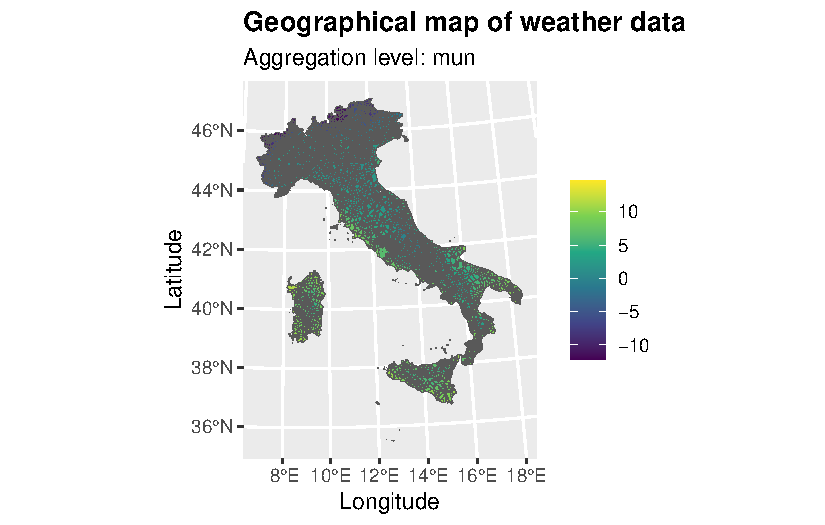
\includegraphics{Demo_guide_files/figure-pdf/unnamed-chunk-8-1.pdf}

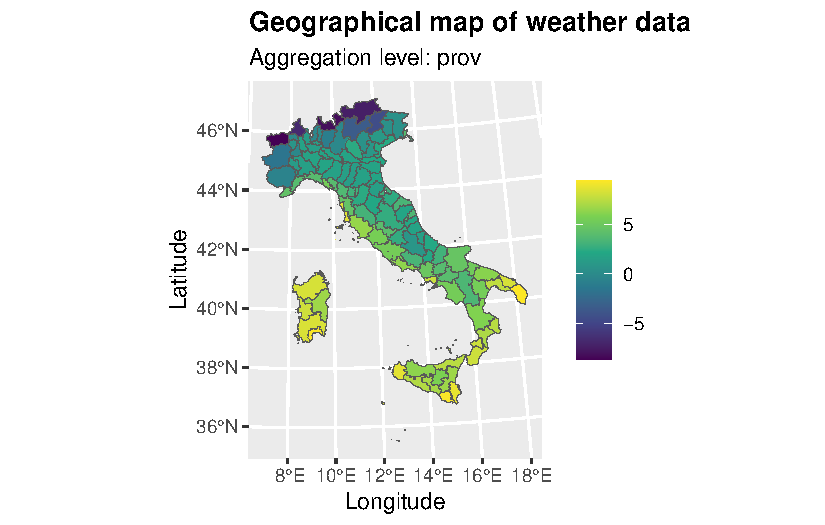
\includegraphics{Demo_guide_files/figure-pdf/unnamed-chunk-8-2.pdf}

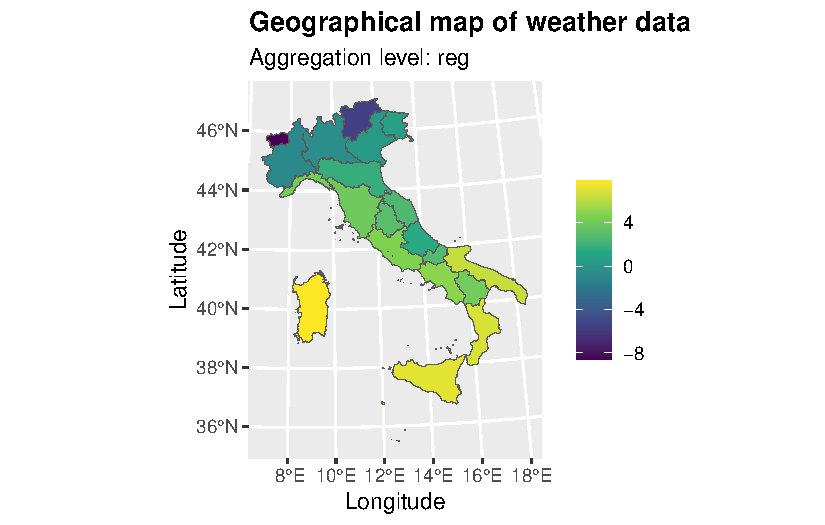
\includegraphics{Demo_guide_files/figure-pdf/unnamed-chunk-8-3.pdf}




\end{document}
